\DiaryEntry{Continuity, Topological Definition}{2016-02-03}{Topology}

\subsection{Open and Closed Intervals}

An open interval \((a,b)\) is defined as the set

\[
(a,b) = \{ x \in \mathcal{R}: a < x < b \}
\]

Note that the open interval does not include the endpoints. A closed
interval does include the end points; i.e.~it is defined as the set

\[
[a,b] = \{ x \in \mathcal{R}: a \leq x \leq b \}
\]

A union of open intervals is not necessarily an open interval again;
e.g. \((0,1) \cup (3,4)\) is not an open interval as it is not possible
to write the union in the form \((a,b)\).

\subsection{Open and Closed Sets}

Instead such a union is called an open set - formally it is defined as:
Let \(\mathcal{S}\) denote a subset of \(\mathcal{R}\). Then
\(\mathcal{S}\) is open, if for every point \(x \in \mathcal{S}\), there
is some open interval \((x-\delta_x, x + \delta_x)\) (\(\delta_x > 0\))
contained in \(\mathcal{S}\).

Consider the example of the open set \(\mathcal{S} = (0,1)\). The point
\(0.1\) is in \(\mathcal{S}\); in addition, we can construct an open
interval \((0.05, 0.15)\) around \(0.1\) which is contained in
\(\mathcal{S}\). Because the endpoints are not included in the open set,
we can continue this argument for any point, no matter how close to the
end point it is: The point \(\epsilon\) (with \(\epsilon \ll 1\)) can
always be surrounded by an open interval \((\epsilon/2, 3\epsilon/2)\),
which is still contained in \(\mathcal{S}\).

In case of an open set this argument is not possible: If we consider a
closed set \(\mathcal{S} = [a,b]\), then we cannot find an open interval
around \(a\) (or \(b\)), which is still contained in \(\mathcal{S}\) -
no matter how small the open interval. The open interval
\((a-\epsilon, a+\epsilon)\) will always be half outside
\(\mathcal{S}\).

Another interpretation of the open interval in the definition above is
that it forms a ``breathing space'' for the point \(x\).

We can repeat above arguments for a union of open intervals and see that
for every point of the intervals, we can find such a breathing space.
Therefore the union of open intervals is an open set.

\subsubsection{Special Cases}

The whole real line \(\mathcal{R}\) is an open set: For every
\(x \in \mathcal{R}\), we can find a neighbourhood which will be
contained in \(\mathcal{R}\).

Conversely, the empty set is also (defined to be) open: There is no
\(x\) around which a breathing space must exist, therefore the set is
open.

\subsubsection{Union and Intersection}

\begin{itemize}
\item
  The union of any collection of open sets is open.
\item
  Any finite intersection of open sets is open. In case of an infinite
  intersection, no general statement is possible.
\end{itemize}

\subsection{Topologial Definition of Continuity}

If \(f: \mathcal{D} \rightarrow \mathcal{C}\) is a function and
\(\mathcal{S}\) is a subset of \(\mathcal{C}\), then the
\textbf{preimage} of \(\mathcal{S}\) under \(f\) is the subset of
\(\mathcal{D}\) defined as all points which get mapped by \(f\) to
\(\mathcal{S}\):

\[
f^{-1}(\mathcal{S}) = \{x \in \mathcal{D}: f(x) \in \mathcal{S} \}
\]

Note that this definition talks about sets (and not single points of a
function) and is therefore quite general.

\subsubsection{Example 1}

As an example, consider the function \(y = f(x) = x^2\). Start with the preimage of a point:

\[
f^{-1}(4) = \{-2, 2\}
\]

Both \(x=2\) and \(x=-2\) get mapped to the value \(y = 4\).

Now consider the preimage of the set \([1,4]\)

\[
f^{-1}([1,4]) = [-2,-1] \cup [1,2]
\]

In a similar spirit we have

\[
f^{-1}((1,4) = (-2,-1) \cup (1,2)
\]

Finally, the preimage can also be empty; for example

\[
f^{-1}(-1) = \{\}
\]

as no real input of \(f(x) = x^2\) yields a function value of \(y=-1\).

Using the preimage concept, we can state the open-set approach to
continuity as follows: Consider a function
\(f: \mathcal{R} \rightarrow \mathcal{R}\) and a subset \(\mathcal{S}\)
of \(\mathcal{R}\). If \(f\) is continuous, then \(f^{-1}(\mathcal{S})\)
is open when \(\mathcal{S}\) is open. Conversely, if
\(f^{-1}(\mathcal{S})\) is open whenever \(\mathcal{S}\) is open, then
\(f\) is continuous.

As an example, consider the function

\[
f(x) = \begin{cases}
x & \mbox{if } x \leq 0 \\
1+x & \mbox{if } x > 0 \end{cases}
\]

shown below.

\begin{figure}
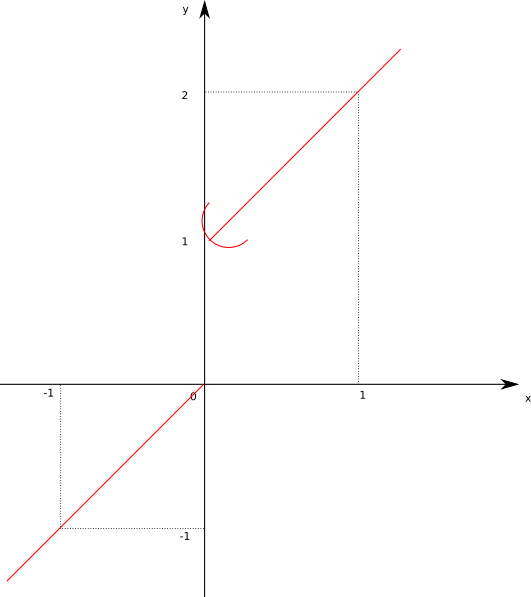
\includegraphics[scale=0.7]{images/continuity_top_01.png}
\end{figure}

The preimage of \((-1,1/2)\) is

\[
f^{-1}((-1,1/2)) = (-1,0]
\]

This is not an open set and therefore the function is not continuous.

\subsubsection{Example 2}

This
\href{http://math.stackexchange.com/questions/287574/proving-continuity-using-the-topological-definition}{post}
considers a function defined as

\[
f(x) = \begin{cases}
0 & x \in \mathcal{R} - \{c\} \\
1 & x = c \end{cases}
\]

i.e. \(f(x)\) is zero everywhere but at \(x=c\) (where it equals 1). Now
consider the open set \(\mathcal{U} = (1/2, 3/2)\) for which the
preimage is \(f^{-1}(\mathcal{U}) = \{c\}\). The preimage is a single
value which is \textbf{not} an open set. Therefore the function is not
continuous.

\subsubsection{Example 3}

This
\href{http://math.stackexchange.com/questions/1340774/intuition-on-the-topological-definition-of-continuity-considering-the-special-c}{post}
deals with the step function defined as

\[
f(x) = \begin{cases}
0 & x \leq 0 \\
1 & x > 0 \end{cases}
\]

Consider the open set \(\mathcal{U} = (-1/2, 1/2)\) with preimage
\(f^{-1}(\mathcal{U}) = (- \infty, 0]\). The set is closed on the right
side, because \(f(0) = 0\). The preimage is not open, therefore the
function is no continuous.
